\documentclass[10pt]{article}
\usepackage[a4paper,margin=2.3cm]{geometry}
\usepackage[utf8]{inputenc}
\usepackage[T1]{fontenc}
\usepackage{lmodern}
\usepackage{microtype}
\usepackage{graphicx}
\usepackage{booktabs}
\usepackage{amsmath}
\usepackage[hidelinks]{hyperref}
\usepackage[parfill]{parskip}

\newcommand{\mse}{\mathrm{MSE}}
\newcommand{\Om}{\bar{\omega}}

\title{\textbf{Differentiable hybrid closure for two-dimensional turbulence:\\composing a PyTorch CNN with a JAX spectral solver across Tesseracts}}
\author{Tesseract Hackathon 2026, Track 3: Hybrid ML + mechanistic models\\[2pt]
\small Repository: \url{https://github.com/julian-8897/tesseract-hybrid-closure}}
\date{31 August 2026}

\begin{document}
\maketitle

\section*{Problem and setting}

Coarse-grid turbulence closure is a standing bottleneck in large-eddy simulation and coupled modelling: a solver that cannot resolve the small scales must still account for their effect on the resolved field. We train a learned subgrid closure for freely decaying two-dimensional vorticity on a $2\pi$-periodic domain. A $256^2$ direct numerical simulation (DNS) provides filtered ground truth for a $64^2$ coarse solver, and we ask whether a closure trained \emph{a-posteriori}, with gradients propagated through the coarse solver trajectory, beats matched alternatives at long rollout rather than at one step only.

\section*{Method}

One hybrid step on the coarse vorticity $\omega_n$ is an operator split:

\begin{equation}
  \omega^* = S_{\mathrm{JAX}}(\omega_n; \Delta t), \qquad
  q_\theta = C_{\mathrm{Torch}}(\omega^*; \theta), \qquad
  \omega_{n+1} = \omega^* + \Delta t\, q_\theta .
\end{equation}

$S_{\mathrm{JAX}}$ is an Exponax ETDRK2 step (JAX), and $C_{\mathrm{Torch}}$ is a ten-layer periodic PyTorch CNN with 822{,}977 flattened parameters that predicts the scalar vorticity tendency. States are float32 arrays of shape $(1,64,64)$. The solver contract is $\omega \to \omega_{\mathrm{next}}$ with JVP and VJP; the closure contract is $(\omega, \theta_{\mathrm{flat}}) \to q_\theta$ with a parameter/state VJP. JVP and VJP are forward- and reverse-mode differentiation (Jacobian-vector and vector-Jacobian products). The two components expose typed contracts; \texttt{tesseract-jax} composes both into one differentiable objective. No finite-difference gradient or surrogate backward model is used.

A-posteriori training minimises the rollout vorticity MSE

\begin{equation}
  L_H(\theta) = \frac{1}{H \cdot 64^2} \sum_{t=1}^{H} \bigl\| \hat{\omega}_t(\theta) - \Om_t^{\mathrm{DNS}} \bigr\|_2^2 ,
\end{equation}

over unrolls $H = 1 \to 5 \to 30$ (Adam, learning rate $10^{-4}$, 700 updates). The matched a-priori baseline instead minimises the one-step squared difference between the closure tendency $q_\theta(\omega^*)$ and the filtered DNS residual tendency, with the target detached from the computation graph, so no solver gradient flows. The baseline shares the architecture, initialisation, optimiser, update budget, train seeds and flow regime; only the objective differs. The comparison therefore measures the benefit of trajectory-aware optimisation in this setting, not a general property of a-priori closures.

\begin{figure}[t]
  \centering
  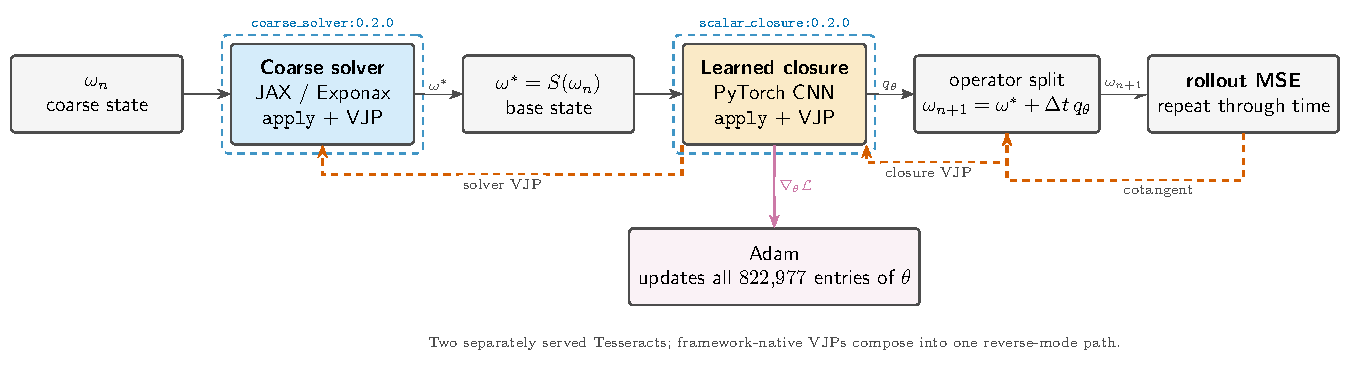
\includegraphics[width=0.92\textwidth]{figures/fig_tesseract_gradient_path.pdf}
  \caption{Forward state and tendency flow through the separately served JAX solver and PyTorch closure Tesseracts; reverse mode returns the closure parameter gradient through the closure VJP and the solver VJP.}
\end{figure}

\section*{Why Tesseract}

The reverse path of record implements the same reverse-mode composition training uses: \texttt{jax.vjp} through Exponax for the solver, PyTorch autograd for the closure, composed into one objective. An ablation verifies that the solver VJP materially shapes the parameter gradient: zeroing its state cotangent at the served endpoint changes a two-step parameter gradient by 39.98\% relative (\texttt{docs/results/container-optimiser-demo.json}), so the solver transpose contributes materially to the parameter gradient. The demo records every endpoint call and fails closed without solver-VJP evidence.

Without this component boundary, the practical alternatives were a monolithic program that couples the two frameworks' dependency trees and reimplements one component in the other's language, or a hand-written AD tape across the boundary that neither framework owns. Here each component stays in its native framework and container and exposes an inspectable, typed contract; the same composed step and derivative contracts run in-process for throughput or as two served images, while the recorded runs differ in unroll objective and update budget (Results).

\section*{Results}

On 32 locked test trajectories rolled to 500 coarse steps, the selected a-posteriori CNN reduces mean 500-step MSE by 71.7\% relative to the no-closure solver and by 15.7\% relative to the matched a-priori CNN. It wins on all 32 seeds at every reported horizon, and every trajectory of every method remains finite through step 500.

\begin{table}[h]
  \centering
  \small
  \begin{tabular}{lccccc}
    \toprule
    Method & 30 steps & 60 steps & 120 steps & 250 steps & 500 steps \\
    \midrule
    A-posteriori CNN (selected) & 0.007280 & 0.02742 & 0.1086 & 0.4458 & \textbf{1.1468} \\
    A-priori CNN, matched        & 0.007622 & 0.02980 & 0.1235 & 0.5234 & 1.3602 \\
    No closure                  & 0.07776  & 0.2777  & 0.9048  & 2.4622  & 4.0516 \\
    Dynamic Smagorinsky         & 0.07796  & 0.2723  & 0.8541  & 2.1910  & 3.3942 \\
    Static Smagorinsky, $C_s{=}0.17$ & 0.08806 & 0.2956 & 0.8682 & 2.0365 & 2.9443 \\
    \bottomrule
  \end{tabular}
  \caption{Mean rollout vorticity MSE over 32 test seeds; per-seed values, standard deviations and paired wins are in the tracked report. Lower is better.}
\end{table}

Diagnostics on the validation split support a physical reading beyond the headline metric. The a-posteriori model is spectrally closer to filtered DNS than the matched a-priori model at every measured step, while dynamic Smagorinsky retains the lowest 500-step enstrophy log-distance (0.2787 against 0.3019) despite a roughly three times larger 500-step validation vorticity MSE: spectral shape and trajectory accuracy separate at long rollout. The spectral distance is the mean absolute log-ratio over shells $1 \le k \le 32$; an endpoint amplitude/phase decomposition at step 500 gives amplitude and phase contributions of 1.2297 and 1.1461 for the selected model, the lowest of the five methods on both terms.

The same composition trains through two transports. The submitted model used the in-process transport for throughput; a 500-update run with every gradient crossing the two served images reduces 30-step validation MSE from 0.085425 to 0.009446 (88.9\%) on the eight held-out validation seeds 10000--10007; the submitted checkpoint scores 0.008248 on those seeds, scored identically (Figure~\ref{fig:served}). A second run trains 100 updates at the locked 30-step unroll entirely through the images (0.085425 to 0.036354, 57.4\%, with 2,900 solver and 3,000 closure VJP calls). Neither served run touches a test seed; both are demonstrations of the deployment boundary, not the submitted model.

\begin{figure}[h]
  \centering
  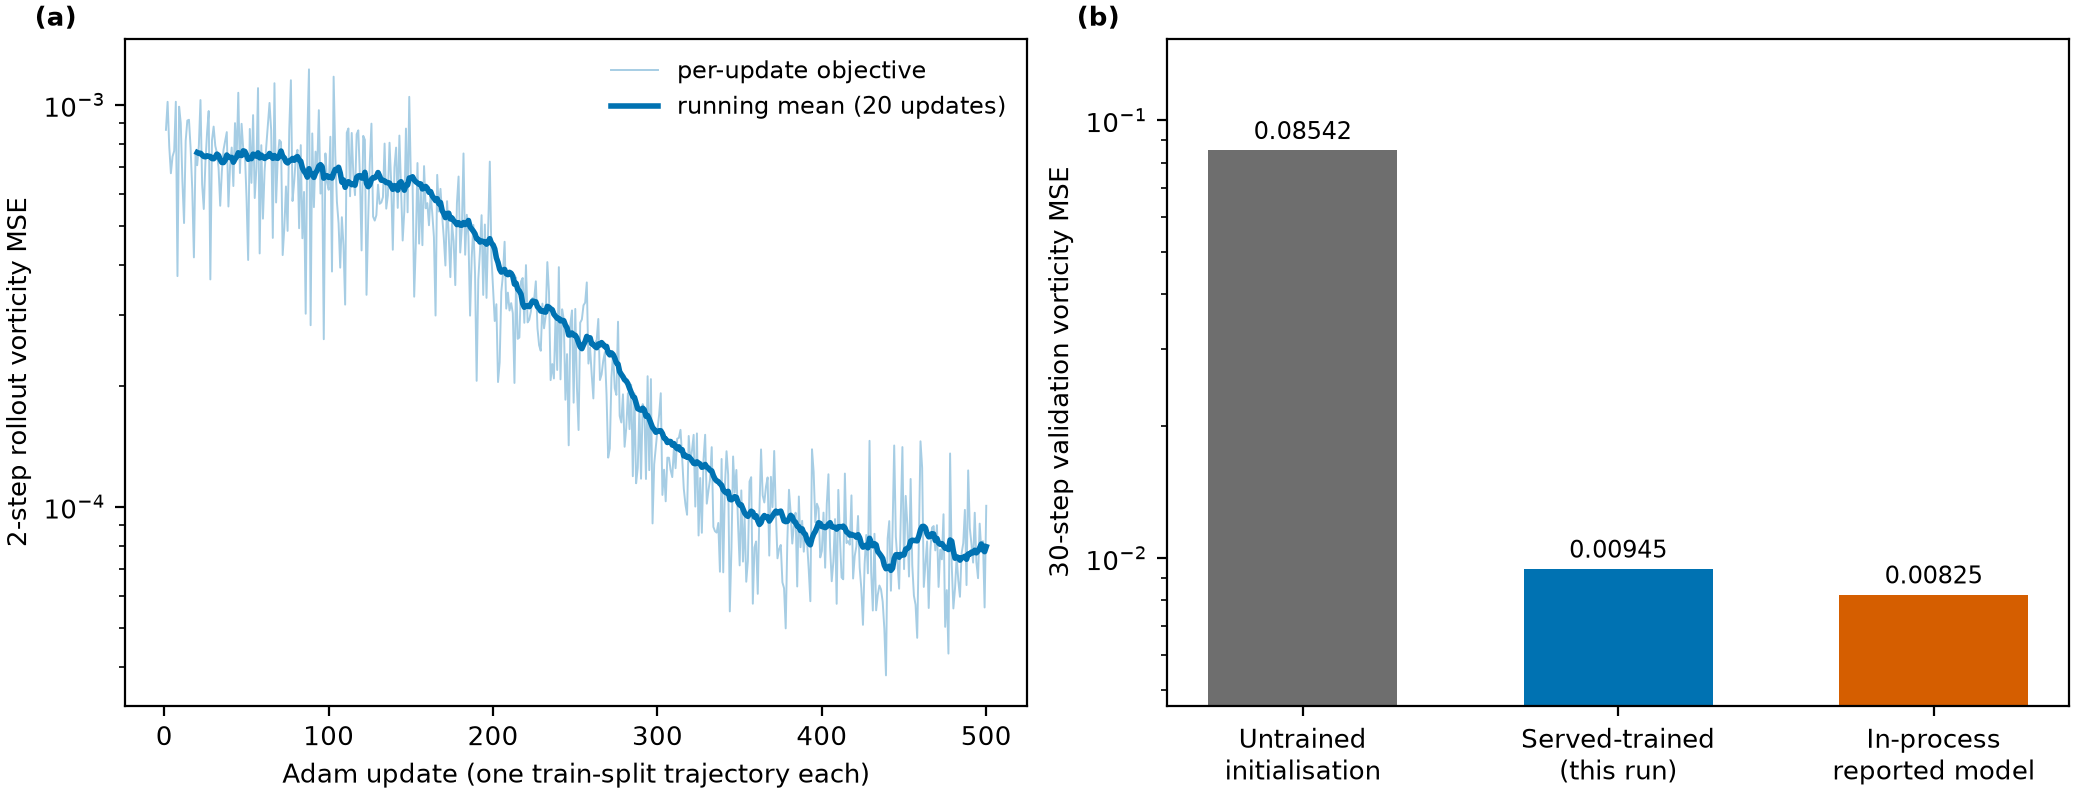
\includegraphics[width=0.92\textwidth]{figures/fig_served_training.png}
  \caption{Training through the served transport. Left: the two-step rollout objective per Adam update for a 500-update run whose every gradient crossed the two served images. Right: 30-step validation MSE on the same eight held-out seeds for the run's initialisation, its endpoint, and the submitted in-process checkpoint, all scored identically.}
  \label{fig:served}
\end{figure}

\begin{figure}[h]
  \centering
  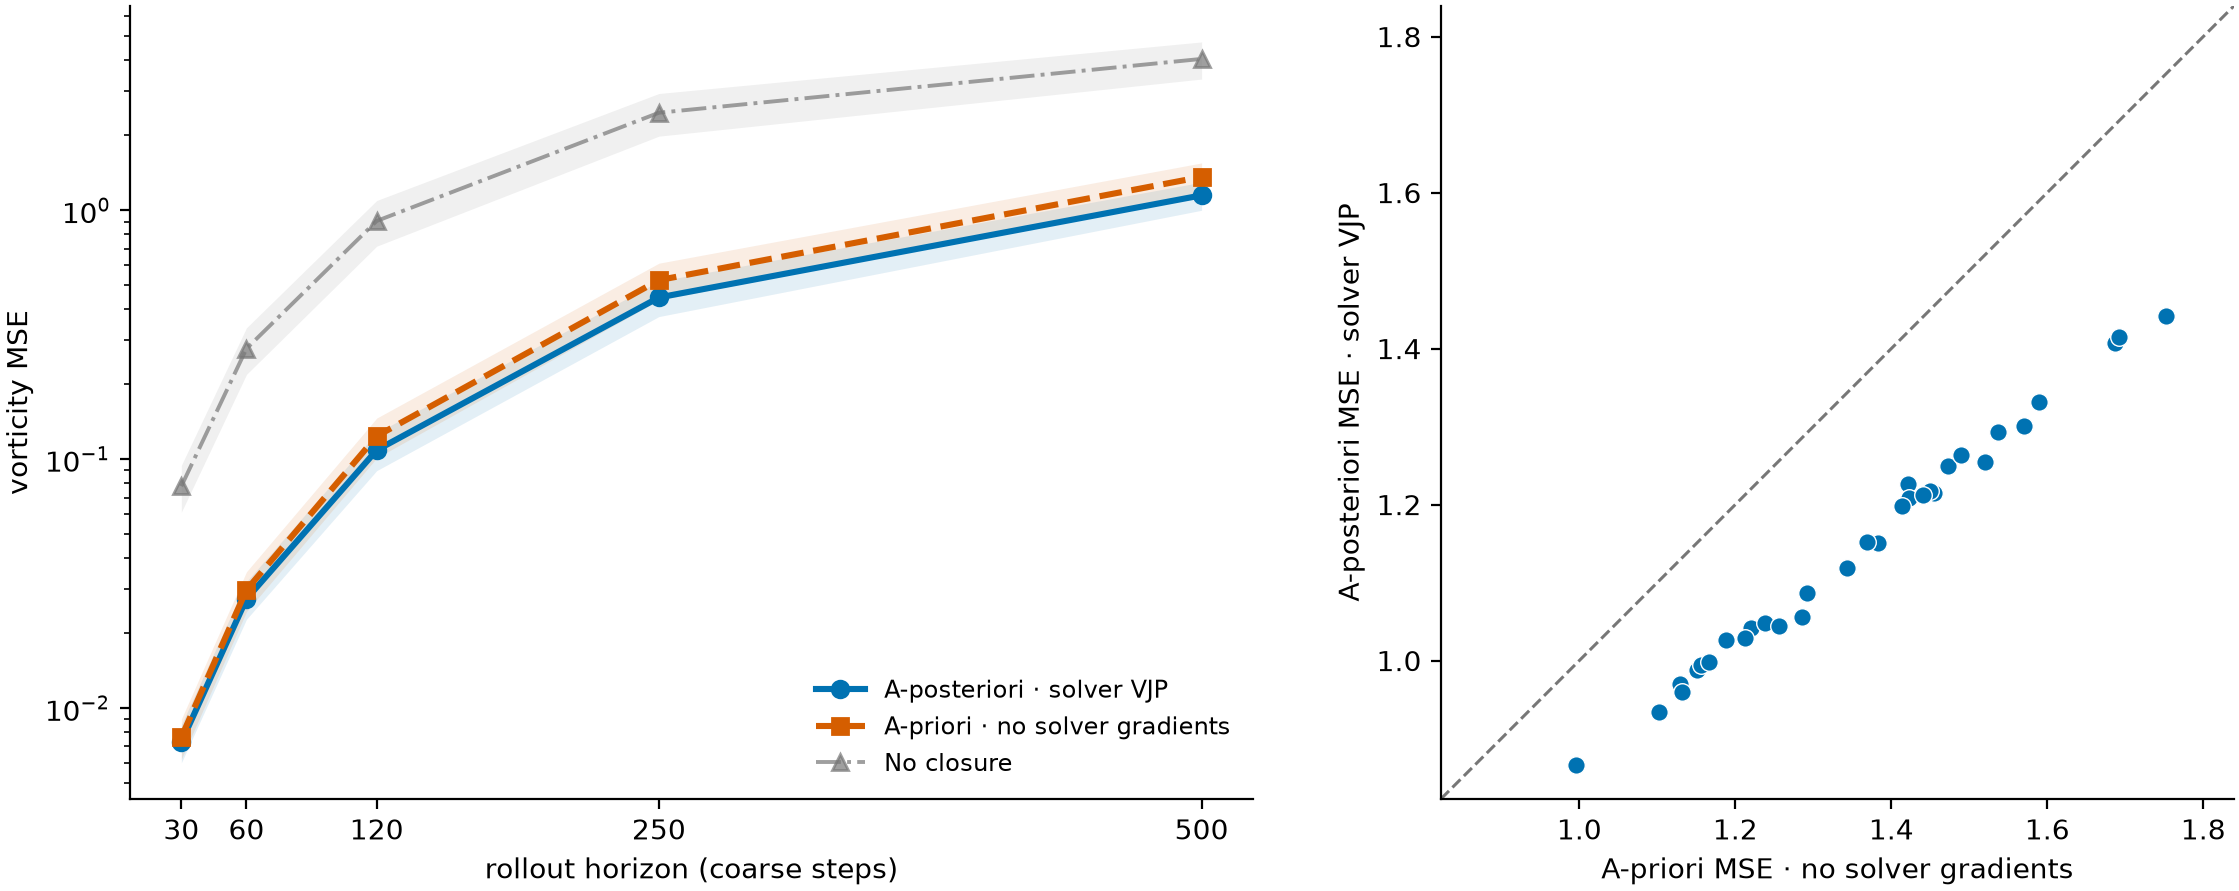
\includegraphics[width=0.80\textwidth]{figures/fig_tesseract_results.png}
  \caption{Left: rollout vorticity MSE of the selected model against the matched a-priori model and the no-closure solver; bands are $\pm 1$ population standard deviation over 32 seeds. Right: paired 500-step errors; every seed lies below the equal-error line.}
\end{figure}

\section*{Protocol, evidence and limitations}

The protocol was fixed before test evaluation: Gaussian random-field initial conditions on a $256^2$ DNS, sharply filtered to $64^2$ coarse truth, with radial modes $10 \le |k| \le 32$ rescaled to $|\omega|_{\max} = 20$; float32 ETDRK2, $\nu = 10^{-3}$, $\Delta t = 0.002$; disjoint seed splits (train 0--9999, validation 10000--10031, test 20000--20031); model selection on mean 30-step validation MSE before the test split was opened. Every aggregate and per-seed value, plus the SHA-256 of the checkpoints and reports behind it, is tracked in \href{https://github.com/julian-8897/tesseract-hybrid-closure/blob/main/docs/results/final-metrics.json}{\texttt{docs/results/final-metrics.json}}, whose digests are post-evaluation integrity evidence. The exact submitted parameters are published as release \href{https://github.com/julian-8897/tesseract-hybrid-closure/releases/tag/submission-2026-08-31}{\texttt{submission-2026-08-31}} (a-posteriori SHA-256 \texttt{8ed5b36f\dots}, a-priori SHA-256 \texttt{8862fbd5\dots}), so a clean clone evaluates the model without retraining, and \href{https://github.com/julian-8897/tesseract-hybrid-closure/blob/main/docs/VERIFICATION.md}{\texttt{docs/VERIFICATION.md}} records what has actually been run, including defects found by review and fixed.

Limitations bound the claims. The evidence covers one freely decaying two-dimensional regime; transfer to forced, stationary or three-dimensional turbulence is untested. The scalar tendency closure has no explicit conservation or dissipativity guarantee, and optimisation uses vorticity MSE only, with spectra measured as diagnostics. The Smagorinsky baselines are fixed formulations rather than tuned competitors. The reported model's parameters were produced through the in-process transport of the same composition; the served transports in Results are deployment-boundary demonstrations.

\section*{References}

\begin{enumerate}
  \item Frezat, H., Le Sommer, J., Fablet, R., Balarac, G. \& Lguensat, R. A posteriori learning for quasi-geostrophic turbulence parametrization. \emph{Journal of Advances in Modeling Earth Systems} (2022). \url{https://arxiv.org/abs/2204.03911}, \url{https://doi.org/10.1029/2022MS003124}.
  \item Guan, Y., Chattopadhyay, A., Subel, A. \& Hassanzadeh, P. Stable a posteriori LES of 2D turbulence using convolutional neural networks: backscattering analysis and generalization to higher Re via transfer learning. \emph{Journal of Computational Physics} \textbf{458}, 111090 (2022). \url{https://arxiv.org/abs/2102.11400}, \url{https://doi.org/10.1016/j.jcp.2022.111090}.
  \item Shankar, V. et al. Differentiable turbulence. \url{https://arxiv.org/abs/2307.03683}.
  \item K\"ohler, F. From numerical simulators of PDEs to neural emulators and back. PhD thesis, TU Munich (2026). \url{https://arxiv.org/abs/2608.24547}.
\end{enumerate}

\end{document}